\documentclass{article}

\usepackage{hyperref} %BUG if put after
\usepackage{tikz}
\usetikzlibrary{calc,shapes,positioning}
\usetikzlibrary{arrows}
\newcommand{\midarrow}{\tikz \draw[-triangle 90] (0,0) -- +(.1,0);}
% Be sure to use PDxF Latex
\pdfoutput=1

\usepackage[latin1]{inputenc}

\usepackage{url}
\usepackage{fullpage}
\usepackage{cite}
\usepackage{caption}
\usepackage{bm}
\newcommand{\ubar}[1]{\mkern2mu\underline{\mkern-2mu #1\mkern-2mu}\mkern2mu}
% \allowdisplaybreaks
\usepackage{mystyle}
\newcommand{\ubm}[1]{\ubar{\bm{#1}}}
\newcommand{\ubmr}[2]{\ubar{\bm{#1}}^{(#2)}}


% \newcommand{\bmtr}[3]{\bm{#1}^{(#3)}_{#2}}

\newcommand{\bmtr}[3]{\bm{#1}^{(#3)}_{#2}}
\newcommand{\smtr}[3]{{#1}^{(#3)}_{#2}}


\usepackage{amsmath,graphicx}
% format A4
% \usepackage{vmargin}
% \setpapersize{A4} 

\RequirePackage{algorithm}
\RequirePackage{algorithmic}

% Attempt to make hyperref and algorithmic work together better:
% \newcommand{\theHalgorithm}{\arabic{algorithm}}


\graphicspath{{./images/}}


\hypersetup{  
  bookmarks=true,
  backref=true,
  pagebackref=false,
  colorlinks=true,
  linkcolor=blue,
  citecolor=red,
  urlcolor=blue,
  pdftitle={Generative Model HMM},
  pdfauthor={Dong Liu},
  pdfsubject={}
}



\title{Powering Hidden Markov Model by Generative Models}
\author{
  Firsthand Scientists
}

% \name{
% Dong Liu,
% Minh Th�nh Vu,
% Saikat Chatterjee,
% and Lars~K. Rasmussen
% }

%   \address{
%   KTH Royal Institute of Technology, Stockholm, Sweden \\
%   E-mail: \{doli, mtvu, sach, lkra\}@kth.se}

\begin{document}

\maketitle
\section{Notation}
Time is indexed by subscript and sequence is denoted by underline. $\bm{x}_t$ is signal at time $t$. The sequential time is denoted by $\ubar{\bm{x}} = \left[ \bm{x}_1,
  \cdots, \bm{x}_T\right]^{\intercal}$, where $[\cdot]^{\intercal}$ means transpose and $T$ is the length of the sequence.  Sequential signal or clip uses underline notation and is indexed by superscript, for instance $\ubar{\bm{x}}^{(r)}$ means the $r$-th sequential signal, where $r = 1, 2, \cdots, R.$, and $\ubmr{x}{r} = \left[ \bmtr{x}{1}{r}, \bmtr{x}{2}{r}, \cdots, \bmtr{x}{T^{(r)}}{r} \right]$ with length ${T^{(r)}}$. Note different sequential signal $\ubmr{x}{r}$ could have different lengths.

The hypothesis of Hidden Markov Model (HMM): $\Hh := \{\bm{H} | \{\Ss, \bm{q}, A, p(\bm{x}|{s}; \bm{\Phi})\}$,
\begin{itemize}
\item $\Ss$ is the set of states of HMM $\bm{H}$;
\item $\bm{q} = \left[ q_1, q_2, \cdots, q_{|\Ss|}\right]^\intercal$ initial distribution of HMM $\bm{H}$ with $|\Ss|$ is cardinality of $\Ss$, $q_k = p(s=k)$ for random state variable $s$.
\item $A$ is the transition matrix for the HMM $\bm{H}$ of size $|\Ss| \times |\Ss|$.
\item Observable signal density $p({\bm{x}}|{s};\bm{\Phi})$ given hidden state sequence, where $\bm{\Phi}$ is the parameter set that defines this conditional probabilistic model.
\end{itemize}

\section{Problem Statement}
Given a empirical distribution $\hat{p}(\ubm{x}) = \frac{1}{R}\sum_{r=1}^{R} \delta_{\ubmr{x}{r}}(\ubm{x})$. We want to find a probabilistic model such that:
\begin{equation}
  \min KL(\hat{p}(\ubm{x})\| p(\ubm{x}))
\end{equation}
where $KL(\cdot\|\cdot)$ denotes the Kullback-Leibler divergence.

When we use HMM to model the empirical distribution and approach the unknown true distribution, the problem boils down to:
\begin{equation}
  \uargmax{\bm{H} \in \Hh} p(\ubm{X}; \bm{H})
\end{equation}
where $\ubm{X} = \left[ \ubmr{x}{1}, \ubmr{x}{2}, \cdots, \ubmr{x}{R} \right]$ 

The problem can be reformulated as
\begin{equation}\label{eq:ml-of-hmm}
  \uargmax{\bm{H} \in \Hh} \sum_{r=1}^{R}\log\,p(\ubmr{x}{r}; \bm{H})
\end{equation}
for independent identical distributed assumption of $\ubm{x}$.

\section{Proposal}


\begin{figure}[!h]
  \centering
  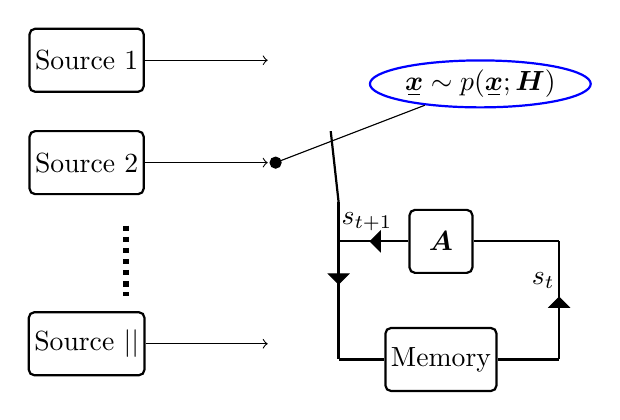
\begin{tikzpicture}
    \tikzstyle{enode} = [thick, draw=blue, ellipse, inner sep = 1pt,  align=center]
    % \tikzstyle{nnode} = [thick, rectangle, rounded corners = 1pt,minimum size = 1.2cm,draw,inner sep = 2pt]
    \tikzstyle{nnode} = [thick, rectangle, rounded corners = 2pt,minimum size = 0.8cm,draw,inner sep = 2pt]
    % \node[enode] (z1) at (-1.2,1.8) {Source 1}; 
    \node[nnode] (g1) at (-0.5,1.8) {Source 1};

    % \node[enode] (z2) at (-1.2,0.5){$\bm{z}\sim p_{2}(\bm{z})$};
    \node[nnode] (g2) at (-0.5,0.5) {Source 2};

    % \node[enode] (zK) at (-1.2,-1.8) {$\bm{z}\sim p_{|\Ss|}(\bm{z})$};
    \node[nnode] (gs) at (-0.5, -1.8) {Source $|\Ss|$};

    \node[enode] (x) at (4.5,1.5){$\ubm{x}\sim p(\ubm{x};\bm{H})$};
    % \node at (3,-1){$p(\bm{z}) = \sum_k\pi_kp_k(\bm{z})$};
    

    \draw[dotted,line width=2pt] (0,-0.3) -- (0,-1.2);
    \filldraw[->] (1.9, 0.5)circle (2pt) --  (x) ;
    
    \draw[->] (g1) -- (1.8, 1.8);

    
    \draw[->] (g2) -- (1.8, 0.5);

    % \draw[->] (1,-0.5) -- (1.8, -0.5);
    
    \draw[->] (gs) -- (1.8, -1.8);

    % \draw[->] (z1) [in=180,out=0]  to node[right]{$\pi_1$} (g);
    % \draw[->] (z2) [in=180,out=0]  to node[above]{$\pi_2$} (g);
    % \draw[->,dashed] (zK) [in=180,out=0]  to node[right]{$\pi_K$} (g);
    % \draw[->] (g) to (x);
    \begin{scope}[xshift=0.5cm, thick, every node/.style={sloped,allow upside down}]
      \node[nnode] (m) at (3.5,-2) {Memory};
      \node[nnode] (a) at (3.5,-0.5) {$\bm{A}$};

      \draw (2.1,0.9)-- (2.2, 0.);
      \draw (2.2,0.)-- node {\midarrow} (2.2,-2);
      \draw (2.2,-2)-- (m);
      \draw (m)-- (5, -2);
      \draw (5, -2)-- node {\midarrow} (5 ,-0.5);
      \draw (5, -0.5) -- (a);
      \draw (a)-- node {\midarrow} (2.2, -0.5);
      \node at (4.8, -1) {$s_{t}$};
      \node at (2.56, -0.25) {$s_{t+1}$};
    \end{scope}
    
    

  \end{tikzpicture}
  \caption{HMM Model defined by $\bm{H} = \{\Ss, \bm{q}, \bm{A}, p({\bm{x}}|{\bm{s}}; \bm{\Phi}) \}$}
  \vspace{0.1cm}
\end{figure}


Since model $\bm{H}$ contains hidden sequential variable $\ubm{s}$, we can not directly solve the maximum likelihood problem in \autoref{eq:ml-of-hmm}. We use expectation maximization (EM) to address the hidden variable problem by
\begin{itemize}
\item E-step: % the posterior probability of $\ubm{s}$:
  % \begin{equation}
  %   p(\ubm{s}|\ubm{x})
  % \end{equation}
  The ``expected likelihood'' function:
  \begin{equation}\label{eq:em-q-funciton}
    \Qq(\bm{H}; \bm{H}^{\mathrm{old}}) = \ \sum_{r=1}^{R}EE_{p(\ubmr{s}{r}| \ubmr{x}{r}; \bm{H}^{\mathrm{old}})}\left[\log\,p(\ubmr{x}{r}, \ubmr{s}{r}; \bm{H}) \right]
  \end{equation}
\item M-step: the optimization step:
  \begin{equation}\label{eq:em-m-opt}
    \umax{\bm{H}} \Qq(\bm{H}; \bm{H}^{\mathrm{old}})
  \end{equation}
\end{itemize}


The \autoref{eq:em-m-opt} can be reformulated as:
\begin{equation}\label{eq:m-step-subs}
  \umax{\bm{H}} \Qq(\bm{H}; \bm{H}^{\mathrm{old}}) = \umax{\bm{q}}\Qq(\bm{q}; \bm{H}^{\mathrm{old}}) + \umax{{A}}\Qq({A}; \bm{H}^{\mathrm{old}}) + \umax{\bm{\Phi}}\Qq(\bm{\Phi}; \bm{H}^{\mathrm{old}})
\end{equation}
where
\begin{align}
  \Qq(\bm{q}; \bm{H}^{\mathrm{old}}) &= \sum_{r=1}^{R} \EE_{p(\ubmr{s}{r}| \ubmr{x}{r}; \bm{H}^{\mathrm{old}})} \left[\log\,p(\smtr{s}{1}{r}; \bm{q})\right] \label{eq:init-distribution-update}\\
  \Qq(\bm{A}; \bm{H}^{\mathrm{old}}) &= \sum_{r=1}^{R} \EE_{p(\ubmr{s}{r}| \ubmr{x}{r}; \bm{H}^{\mathrm{old}})} \left[\log\,\sum_{t=1}^{T^{(r)}-1}p(\smtr{s}{t+1}{r}|\smtr{s}{t}{r}; {A})\right] \label{eq:transition-update}\\
  \Qq(\bm{\Phi}; \bm{H}^{\mathrm{old}}) &= \sum_{r=1}^{R} \EE_{p(\ubmr{s}{r}| \ubmr{x}{r}; \bm{H}^{\mathrm{old}})} \left[\log\,p(\ubmr{x}{r} | \ubmr{s}{r}; \bm{\Phi})\right]\label{eq:generative-model-update}
\end{align}

We can see that the solution of $H$ depends on the posterior probability $p(\ubm{s}| \ubm{x}; \bm{H})$. Though the evaluation of posterior according to Bayesian theorem is simple, the computation complexity of $p(\ubm{s}| \ubm{x}; \bm{H})$ grows exponentially with the length of $\ubm{s}$. Therefore, we would employ Forward/Backward algorithm \cite{} to do the posterior computation efficiently. The marginal $p(s_t| \ubm{x}; \bm{H})$ is also efficiently computed as the joint posterior. 

We summarize the optimization algorithm as:

\begin{algorithm}[H]
  \caption{Meta algorithm for HMM powered by Generative Models}
  \begin{algorithmic}[1]
    \STATE {\bfseries Input:}{
      Building $\bm{H}^{\mathrm{old}}, \bm{H} \in \Hh$ gives: \\
      $\bm{H}^{\mathrm{old}} = \{\Ss, \bm{q}^{\mathrm{old}}, A^{\mathrm{old}}, p(\bm{x}|s; \bm{\Phi}^{\mathrm{old}})\}$, $\bm{H} = \{\Ss, \bm{q}, A, p(\bm{x}|s; \bm{\Phi})\}$
    }, \\
    \STATE Initialize $\bm{H}$
    \STATE $\bm{H}^{\mathrm{old}} \gets \bm{H}$
    \FOR { $\bm{H}$ not converge}
    \STATE Sample a batch of data $\left\{ \ubmr{x}{r} \right\}_{r=1}^{R_b}$ from the dataset $\hat{p}(\ubm{x})$
    \STATE Compute $p(\smtr{s}{t}{r} | \ubmr{x}{r}; \bm{H}^{\mathrm{old}})$, $p(\smtr{s}{t}{r}, \smtr{s}{t+1}{r}| \ubmr{x}{r}; \bm{H}^{\mathrm{old}})$ by forward/backward algorithm;
    \STATE $\bm{q} \gets \uargmin{\bm{q}}\, \Qq(\bm{q}; \bm{H}^{\mathrm{old}})$ by \autoref{eq:update-initial-state-prob};
    \STATE $\bm{A} \gets \uargmin{\bm{A}}\Qq(\bm{A}; \bm{H}^{\mathrm{old}})$ by \autoref{eq:update-transition-prob};
    \STATE $\bm{\Phi} \gets \uargmin{\bm{\Phi}}\Qq(\bm{\Phi}; \bm{H}^{\mathrm{old}})$ by calling Algorithm \autoref{algo:opt-Phi-GenHMM} or \autoref{algo:opt-Phi-LatHMM};
    \STATE $\bm{H}^{\mathrm{old}} \gets \bm{H}$

    \ENDFOR
  \end{algorithmic}
\end{algorithm}


\subsection{Initial Probability Update}
\autoref{eq:init-distribution-update} can be written as:
\begin{align}
  \Qq(\bm{q}; \bm{H}^{\mathrm{old}}) &= \sum_{r=1}^{R}\sum_{\ubmr{s}{r}} {p(\ubmr{s}{r}| \ubmr{x}{r}; \bm{H}^{\mathrm{old}})} \log\,p(\smtr{s}{1}{r}; \bm{q}) \nonumber \\
                                     & = \sum_{r=1}^{R}\sum_{\smtr{s}{1}{r}=1}^{|\Ss|}\sum_{\smtr{s}{2}{r}=1}^{|\Ss|}\cdots \sum_{\smtr{s}{T^{r}}{r}}^{{|\Ss|}} {p(\smtr{s}{1}{r}, \smtr{s}{2}{r}, \cdots, \smtr{s}{T^{r}}{r}| \ubmr{x}{r}; \bm{H}^{\mathrm{old}})} \log\,p(\smtr{s}{1}{r}; \bm{q}) \\
                                     & = \sum_{r=1}^{R}\sum_{\smtr{s}{1}{r}=1}^{|\Ss|}{p(\smtr{s}{1}{r}| \ubmr{x}{r}; \bm{H}^{\mathrm{old}})} \log\,p(\smtr{s}{1}{r}; \bm{q}) 
\end{align}

Since $p(\smtr{s}{1}{r}; \bm{H})$ is the probability of initial state of HMM $\bm{H}$ for $r$-th sequential, actually $q_i = p(\smtr{s}{1}{r} =i;\bm{H} ) $ for $i= 1, 2, \cdots, |\Ss|$. Solution to problem:
\begin{align}
  \bm{q}^{\mathrm{new}} &= \uargmax{\bm{q}} \Qq(\bm{q}; \bm{H}^{\mathrm{old}}), \nonumber \\
                        &\mathrm{s.t.} \sum_{i=1}^{ |\Ss| }q_i = 1 \nonumber\\
                        &q_i \geq 0, \forall s.
\end{align}
is
\begin{equation}\label{eq:update-initial-state-prob}
  q_i = \frac{1}{R} \sum_{r=1}^{R} p(\smtr{s}{1}{r}=i | \ubmr{x}{r}; \bm{H}^{\mathrm{old}}), \forall\; i = 1, 2, \cdots, |\Ss|.
\end{equation}

\subsection{Transition Probability Update}
\autoref{eq:transition-update} can be written as
\begin{align}
  \Qq(\bm{A}; \bm{H}^{\mathrm{old}})
  &= \sum_{r=1}^{R} \EE_{p(\ubmr{s}{r}| \ubmr{x}{r}; \bm{H}^{\mathrm{old}})} \left[\log\,\sum_{t=1}^{T^{(r)}-1}p(\smtr{s}{t+1}{r}|\smtr{s}{t}{r}; {A})\right] \nonumber\\
  &= \sum_{r=1}^{R} \sum_{\ubmr{s}{r}}{p(\ubmr{s}{r}| \ubmr{x}{r}; \bm{H}^{\mathrm{old}})} \log\,\sum_{t=1}^{T^{(r)}-1}p(\smtr{s}{t+1}{r}|\smtr{s}{t}{r}; {A}) \nonumber \\
  &= \sum_{r=1}^{R} \sum_{t=1}^{T^{(r)}-1} \sum_{\smtr{s}{t}{r}=1}^{|\Ss|}\sum_{\smtr{s}{t+1}{r}=1}^{|\Ss|}{p(\smtr{s}{t}{r}, \smtr{s}{t+1}{r}| \ubmr{x}{r}; \bm{H}^{\mathrm{old}})} \log\,p(\smtr{s}{t+1}{r}|\smtr{s}{t}{r}; {A})
\end{align}

Since $\bm{A}_{i, j}  = p(\smtr{s}{t+1}{r}=j|\smtr{s}{t}{r}=i; {A})$ where $A_{i, j}$ is the element of transition matrix $A$, the solution to problem:
\begin{align}\label{eq:update-transition-prob}
  \bm{A}^{\mathrm{new}} = &\uargmax{\bm{A}} \Qq(\bm{A}; \bm{H}^{\mathrm{old}}), \nonumber \\
  \mathrm{s.t.} &\hspace{0.2cm} \bm{A} \cdot \bm{1} = \bm{1} \nonumber \\
                          &  \bm{A}^{\intercal} \cdot \bm{1} = \bm{1} \nonumber \\
                          & \bm{A}_{i,j} \geq 0.
\end{align}
is
\begin{equation}
  \bm{A}_{i,j}^{\mathrm{new}} = \frac{\bar{\xi}_{i,j}}{\sum_{k = 1}^{|\Ss|} \bar{\xi}_{i,k}},
\end{equation}
where
\begin{equation}
  \bar{\xi}_{i,j} = \sum_{r= 1}^{R} \sum_{t= 1}^{T^{(r)}-1}{p(\smtr{s}{t}{r}=i, \smtr{s}{t+1}{r}=j| \ubmr{x}{r}; \bm{H}^{\mathrm{old}})}
\end{equation}

\subsection{Generative Model Update}
\autoref{eq:generative-model-update} can be rewritten as
\begin{align}\label{eq:gm-update}
  \Qq(\bm{\Phi}; \bm{H}^{\mathrm{old}})
  &= \sum_{r=1}^{R}\sum_{\ubmr{s}{r}}{p(\ubmr{s}{r}| \ubmr{x}{r}; \bm{H}^{\mathrm{old}})} \log\,p(\ubmr{x}{r} | \ubmr{s}{r}; \bm{\Phi}) \nonumber \\
  &= \sum_{r=1}^{R} \sum_{t=1}^{{T}^{(r)}-1} \sum_{\smtr{s}{t}{r}=1}^{|\Ss|}  p(\smtr{s}{t}{r}| \ubmr{x}{r}; \bm{H}^{\mathrm{old}}) \log\, p(\bmtr{x}{t}{r} | \smtr{s}{t}{r}; \bm{\Phi}).
\end{align}

Then the third subproblem of \autoref{eq:m-step-subs} becomes:
\begin{align}\label{eq:sub-gm}
  &\uargmax{\bm{\Phi}} \Qq(\bm{\Phi}; \bm{H}^{\mathrm{old}}), \nonumber \\
  \mathrm{s.t.} &\hspace{0.2cm} p(\bm{x} | {s}; \bm{\Phi}) \mathrm{~is~our~ general~model}
\end{align}

It could be seen from \autoref{eq:gm-update} that the key to update generate  model is to evaluate $p(\bm{x}|{s}; \bm{\Phi})$ for all $s \in \Ss$. In Forward/Backward algorithm, evaluation of $p(\bm{x}|{s}; \bm{\Phi})$ is also all what is needed to compute $p(s|\bm{x};\bm{\Phi})$. In the following two subsections, we will provide two neural network based generative models that fulfill this requirement and also have high capability for complex signal modeling.



\subsubsection{Generator Mixed HMM (GenHMM)}\label{subsubsec:GenHMM}
\begin{figure}[!h]
  \centering
  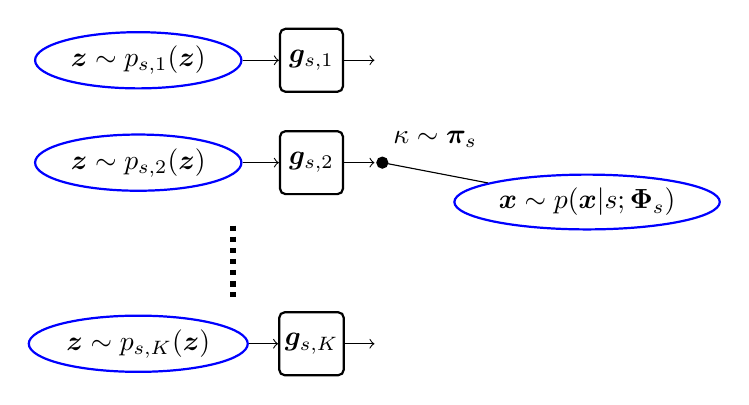
\begin{tikzpicture}
    % \tikzstyle{enode} = [thick, draw=blue, circle, inner sep = 3pt,
    % align=center]
    \tikzstyle{enode} = [thick, draw=blue, ellipse, inner sep = 2pt,  align=center]
    \tikzstyle{nnode} = [thick, rectangle, rounded corners = 2pt,minimum size = 0.8cm,draw,inner sep = 2pt]

    \node[enode] (z1) at (-1.2,1.8) {$\bm{z}\sim p_{s,1}(\bm{z})$};
    \node[nnode] (g1) at (1,1.8) {$\bm{g}_{s,1}$};

    \node[enode] (z2) at (-1.2,0.5){$\bm{z}\sim p_{s,2}(\bm{z})$};
    \node[nnode] (g2) at (1,0.5) {$\bm{g}_{s,2}$};

    \node[enode] (zK) at (-1.2,-1.8) {$\bm{z}\sim p_{s,K}(\bm{z})$};
    \node[nnode] (gs) at (1, -1.8) {$\bm{g}_{s,K}$};

    \node[enode] (x) at (4.5,0){$\bm{x}\sim p(\bm{x}| s; \bm{\Phi}_{s})$};
    % \node at (3,-1){$p(\bm{z}) = \sum_k\pi_kp_k(\bm{z})$};
    

    \draw[dotted,line width=2pt] (0,-0.3) -- (0,-1.2);
    \filldraw[->] (1.9, 0.5)circle (2pt) --  node[above=0.2]{${\kappa}\sim \bm{\pi}_{s}$} (x)  ;
    \draw[->] (z1) -- (g1);
    \draw[->] (g1) -- (1.8, 1.8);

    \draw[->] (z2) -- (g2);
    \draw[->] (g2) -- (1.8, 0.5);

    % \draw[->] (1,-0.5) -- (1.8, -0.5);
    \draw[->] (zK) -- (gs);
    \draw[->] (gs) -- (1.8, -1.8);


    % \node[enode] (z) at (0,0) {$\bm{z}\sim p(\bm{z})$};
    % \node[enode] (x) at (5.5,0){$\bm{x}\sim p(\bm{x}; \bm{\Phi})$};
    %               % \node at (5.2,-1) {$p(\bm{x};\bm{\Phi}) = \textstyle\sum_{k=1}^K \pi_k  p_k(\bm{x})$};
    % \node[nnode] (g1) at (2.6,1.8) {$\bm{g}_1$};
    % \node[nnode] (g2) at (2.6,0.5) {$\bm{g}_2$};
    % \node[nnode] (gk) at (2.6,-1.8) {$\bm{g}_K$};
    % \draw[dotted,line width=2pt] (2.6,-0.3) -- (2.6,-1.2);
    % \draw[->] (z) [in= 180, out =0] to (g1);
    % \draw[->] (z) [in= 180, out =0] to (g2);
    % \draw[->] (z) [in= 180, out =0] to (gk);
    % \filldraw[->] (3.7, 0.5)circle (2pt) -- node[above=0.2]{$\bm{s}\sim \bm{\pi}$} (x) ;
    %               % \draw[->] (3,-0.8) -- (3.5, -0.8);
    % \draw[->] (g1) -- (3.5,1.8);
    % \draw[->] (g2) -- (3.5, 0.5);
    % \draw[->] (gk) -- (3.5, -1.8);
  \end{tikzpicture}
  \caption{Source $s$ powered by generator mixed generative model (GenHMM).}
  \vspace{0.1cm}
\end{figure}

Base on the generative model assumption:

\begin{equation}
  p(\bm{x}| s; \bm{\Phi}_{s}) = \sum_{\kappa=1}^{K}\pi_{s, \kappa} p(\bm{x}| s, \kappa; \bm{\Phi}_{s, \kappa})
\end{equation}
where $\bm{\Phi}_s = \left\{ \bm{\Phi}_{s, \kappa}| \kappa = 1, 2, \cdots, K. \right\}$, and 
\begin{equation}
  \sum_{\kappa = 1}^{K} \pi_{s, \kappa}= 1
\end{equation}

% Let us denote the inverse of $\bm{g}_s$ as $\bm{f}_s = \bm{g}_s^{-1}$.
% For this case we assume the latent sources are Gaussian. We write the emission probability model as a $K$ generator mixed model:
% \begin{align}
    %     p(\bm{x} | s; \bm{\Phi}) &= \sum_{\kappa = 1}^{K} \pi_{s, \kappa} \Nn\left( \bm{f}_{s,\kappa}(\bm{x}); \bm{\mu}_{s,\kappa}, \bm{C}_{s,\kappa}  \right)\bigg|\det\,\left( \pd{\bm{f_{s,\kappa}(\bm{x})}}{\bm{x}} \right)\bigg| \nonumber \\
    %     \sum_{\kappa = 1}^{K} \pi_{s, \kappa}&= 1
                                                 %   \end{align}

The help function should be revised to deal with the new latent variable $\kappa$ into:
\begin{align}\label{eq:obj-q-gen-mix}
  \Qq(\bm{\Phi}; \bm{H}^{\mathrm{old}}) & = \sum_{r=1}^{R} \sum_{t=1}^{{T}^{(r)}-1} \sum_{\smtr{s}{t}{r}=1}^{|\Ss|} \sum_{\smtr{\kappa}{t}{r}=1}^{K}p(\smtr{s}{t}{r}, \smtr{\kappa}{t}{r}| \ubmr{x}{r}; \bm{H}^{\mathrm{old}})  \log\,p(\smtr{\kappa}{t}{r}, \bmtr{x}{t}{r}| \smtr{s}{t}{r}; \bm{\Phi})\nonumber \\
  =& \sum_{r=1}^{R} \sum_{t=1}^{{T}^{(r)}-1} \sum_{\smtr{s}{t}{r}=1}^{|\Ss|}  \sum_{\smtr{\kappa}{t}{r}=1}^{K}p(\smtr{s}{t}{r}| \ubmr{x}{r}; \bm{H}^{\mathrm{old}})p(\smtr{\kappa}{t}{r}|\smtr{s}{t}{r}, \ubmr{x}{r}; \bm{H}^{\mathrm{old}}) \bigg[\log\,\pi_{\smtr{s}{t}{r},\smtr{\kappa}{t}{r}} \nonumber \\
                                        & + \log\, p(\bmtr{x}{t}{r} | \smtr{s}{t}{r}, \smtr{\kappa}{t}{r}; \bm{\Phi}) \bigg]
\end{align}
                                          %                                           \Nn\left( \bm{f}_{\smtr{s}{t}{r},\smtr{\kappa}{t}{r}}(\bm{x}); \bm{\mu}_{\smtr{s}{t}{r},\smtr{\kappa}{t}{r}}, \bm{C}_{\smtr{s}{t}{r},\smtr{\kappa}{t}{r}} \right) \log\,\bigg| \det\, \left( \pd{\bm{f}_{\smtr{s}{t}{r},\smtr{\kappa}{t}{r}}(\bmtr{x}{t}{r})}{\bmtr{x}{t}{r}} \right) \bigg| \bigg].
                                          %   \end{align}
In \autoref{eq:obj-q-gen-mix}, $p(s_t| \ubm{x}, \bm{H}^{\mathrm{old}})$ is computed by forward/backward algorithm. The posterior of $\kappa$ is:
\begin{align}\label{eq:kappa-posterior}
  p(\kappa| s, \ubm{x}; \bm{H}^{\mathrm{old}})
  &=  \frac{p(\kappa, \ubm{x}| s; \bm{H}^{\mathrm{old}})}{p(\ubm{x}| s,\bm{H}^{\mathrm{old}})} \nonumber \\
  & = \frac{\pi_{s, \kappa} p(\ubm{x}| s, \kappa, \bm{H}^{\mathrm{old}})}{\sum_{\kappa=1}^{K} \pi_{s, \kappa} p(\ubm{x}| s, \kappa,\bm{H}^{\mathrm{old}})} \nonumber \\
  & = \frac{\pi_{s, \kappa} p(\bm{x}| s, \kappa, \bm{H}^{\mathrm{old}})}{\sum_{\kappa=1}^{K}  \pi_{s, \kappa} p(\bm{x}| s, \kappa,\bm{H}^{\mathrm{old}})} 
  % & = \frac{\pi_{s_t, \kappa_t} \Nn\left( \bm{f}_{{s}_{t},{\kappa}_{t}}(\bm{x}); \bm{\mu}_{{s}_{t},{\kappa}_{t}}, \bm{C}_{{s}_{t},{\kappa}_{t}} \right) \bigg| \det\, \left( \pd{\bm{f}_{{s}_{t},{\kappa}_{t}}(\bmtr{x}{t}{r})}{\bmtr{x}{t}{r}} \right) \bigg| }{\sum_{\kappa_t=1}^{K}\pi_{s_t, \kappa_t} \Nn\left( \bm{f}_{{s}_{t},{\kappa}_{t}}(\bm{x}); \bm{\mu}_{{s}_{t},{\kappa}_{t}}, \bm{C}_{{s}_{t},{\kappa}_{t}} \right) \bigg| \det\, \left( \pd{\bm{f}_{{s}_{t},{\kappa}_{t}}(\bmtr{x}{t}{r})}{\bmtr{x}{t}{r}} \right) \bigg|} \nonumber \\
\end{align}
where the last equation is due to the fact that only $\bm{x}_t$ among sequence $\ubm{x}$ depends on $s_t, \kappa_t$. 



    %     \begin{align}

    %   \end{align}

The latent prior for mixture of each source $s$ is obtained by solving the following problem:
\begin{align}
  \pi_{s, \kappa} & = \uargmax{pi_{s, \kappa}} \Qq(\bm{\Phi}; \bm{H}^{\mathrm{old}}) \\ \nonumber
                  & s.t. \, \sum_{\kappa=1}^{K} \pi_{s, \kappa}= 1
\end{align}
which gives the solution:
\begin{equation}\label{eq:mix-latent-parameter-solution}
  \pi_{s, \kappa} = \frac{\sum_{r=1}^{R} \sum_{t=1}^{{T}^{(r)}-1} p(\smtr{s}{t}{r} =s, \smtr{\kappa}{t}{r}=\kappa | \ubmr{x}{r}; \bm{H}^{\mathrm{old}}) }{\sum_{k =1}^{K}\sum_{r=1}^{R} \sum_{t=1}^{{T}^{(r)}-1} p(\smtr{s}{t}{r} =s, \smtr{\kappa}{t}{r}=k | \ubmr{x}{r}; \bm{H}^{\mathrm{old}}) }
\end{equation}
where $p(s, \kappa | \ubm{x}; \bm{H}^{\mathrm{old}}) = p(s| \ubm{x}; \bm{H}^{\mathrm{old}}) p(\kappa | s, \ubm{x}; \bm{H}^{\mathrm{old}})$ that can be computed by results of forward/backward and \autoref{eq:kappa-posterior}.

In implementation, GenHMM uses the generator mixed emission model with $\kappa$-th component as:

\begin{align}
  &p(\bm{x}| s, \kappa; \bm{\Phi}_{s, \kappa}) \nonumber \\
  =&p_{s, \kappa}(\bm{z}) \bigg| \det \left( \pd{\bm{z}}{\bm{x}} \right) \bigg| \nonumber \\
  = &\Nn\left( \bm{f}_{{s},{\kappa}}(\bm{x}); \bm{\mu}_{{s},{\kappa}}, \bm{C}_{{s},{\kappa}} \right) \bigg| \det\, \left( \pd{\bm{f}_{{s},{\kappa}}(\bm{x})}{\bm{x}} \right) \bigg|
\end{align}
where $\bm{f}_{{s},{\kappa}} = \bm{g^{-1}_{{s},{\kappa}}}$ is defined by parameter set $\bm{\theta}_{s, \kappa}$, and $\bm{\Phi}_{s, \kappa} = \left\{\bm{\mu}_{{s},{\kappa}}, \bm{C}_{{s},{\kappa}} , \bm{\theta}_{s, \kappa} \right\}, \kappa = 1, 2, \cdots, K$. We can start by setting $\bm{\mu}_{{s},{\kappa}} = \bm{0}$ and $\bm{C}_{{s},{\kappa}} = diag(\bm{1})$.
\begin{algorithm}[H]
  \caption{M-step w.r.t. $\bm{\Phi}$ powered by GenMM}\label{algo:opt-Phi-GenHMM}
  \begin{algorithmic}[1]
    \STATE {\bfseries Input:}
    Latent mixture distribution: $\Nn\left(\bm{z}; \bm{0}, \mathrm{diag}(\bm{1})\right)$, $\forall \, s \in \Ss, \kappa = 1, 2, \cdots, K$;\\
    Empirical distribution $\hat{p}(\bm{x})$ of dataset; \\
    \STATE Set a total number of epochs $T$ of training as stop criterion. A learning rate $\eta$.
    \FOR {epoch $t < T$}
    \STATE Sample a batch of data $\left\{ \ubmr{x}{r} \right\}_{r=1}^{R_b}$ from dataset $P_d(\ubm{x})$
    
    \STATE Compute $p(\smtr{s}{t}{r}, \smtr{\kappa}{t}{r}| \ubmr{x}{r}; \bm{H}^{\mathrm{old}})$  by Forward/backward and \autoref{eq:kappa-posterior}.
    %     = \frac{\pi_k \Nn\left(f(X); \bm{\mu}_k^{t},\bm{\sigma}_k^{t}\right)}{\sum_{k=1}^K\; \pi_k\Nn\left(f(X); \bm{\mu}_k^{t},\bm{\sigma}_k^{t}\right) }, \forall \left\{ x^{(i)}\right\}_{i=1}^{n_b}$
    % \Comment{Calculate posterior \autoref{eq-posterior-gamma}}
    \STATE Compute loss ${\Qq}\left({\bm{\Phi}}, {\bm{H}}^{\mathrm{old}}\right)$ in \autoref{eq:obj-q-gen-mix}

    \STATE $\partial{\bm{\th}_s} \gets  \nabla_{\bm{\theta}} -
    \frac{1}{R_{b}}{\Qq}\left({\bm{\Phi}},{\bm{H}}^{\mathrm{old}}\right)$
    % \Comment{E-step}
    % \STATE $\partial{g_k} \gets \nabla_{\th_k}\widetilde{\Qq}\left(\left\{ \th_k
    %   \right\}_{k=1}^{K};\left\{ \th_k^t\right\}_{k=1}^{K}\right)$,
    % $\forall \th_k \in\left\{ \th_k\right\}_{k=1}^{K}$
    \STATE $\bm{\th}_s \gets \bm{\th}_s - \eta \cdot \partial{\bm{\theta}_s}$, $\forall s \in \Ss$
    \ENDFOR
    
    \STATE Update $\pi_{s, \kappa}, \forall, s\in \Ss, \kappa= 1, 2, \cdots, K$, according to \autoref{eq:mix-latent-parameter-solution}
        
    \STATE Assemble $\bm{\Phi} = \left\{  \bm{\Phi}_s| s \in \Ss\right\}$ for $\bm{\Phi}_s = \left\{ \bm{\theta}_{s, \kappa}, \bm{\mu}_{{s},{\kappa}}, \bm{C}_{{s},{\kappa}}| \kappa = 1, 2, \cdots, K \right\}$.
    
    
  \end{algorithmic}
\end{algorithm}




\subsubsection{Latent-source Mixed HMM (LatMM)}

\begin{figure}[h]
  \centering
  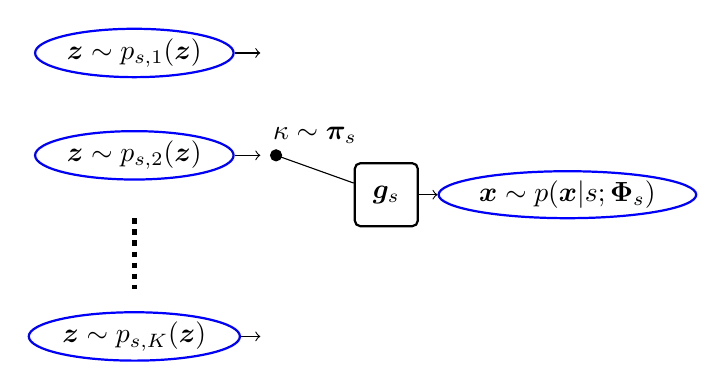
\begin{tikzpicture}
    \tikzstyle{enode} = [thick, draw=blue, ellipse, inner sep = 1pt,  align=center]
    % \tikzstyle{nnode} = [thick, rectangle, rounded corners = 1pt,minimum size = 1.2cm,draw,inner sep = 2pt]
    \tikzstyle{nnode} = [thick, rectangle, rounded corners = 2pt,minimum size = 0.8cm,draw,inner sep = 2pt]
    \node[enode] (z1) at (0,1.8) {$\bm{z}\sim p_{s,1}(\bm{z})$};
    \node[enode] (z2) at (0,0.5){$\bm{z}\sim p_{s,2}(\bm{z})$};
    \node[enode] (zK) at (0,-1.8) {$\bm{z}\sim p_{s, K}(\bm{z})$}; 
    \node[enode] (x) at (5.5,0){$\bm{x}\sim p(\bm{x}|s;{\bm{\Phi}}_{s})$};
    % \node at (3,-1){$p(\bm{z}) = \sum_k\pi_kp_k(\bm{z})$};
    \node[nnode] (g) at (3.2,0) {$\bm{g}_s$};
    \draw[dotted,line width=2pt] (0,-0.3) -- (0,-1.2);
    \filldraw[->] (1.8, 0.5)circle (2pt) -- node[above=0.2]{${\kappa}\sim \bm{\pi}_s$} (g) ;
    \draw[->] (z1) -- (1.6, 1.8);
    \draw[->] (z2) -- (1.6, 0.5);
    % \draw[->] (1,-0.5) -- (1.8, -0.5);
    \draw[->] (zK) -- (1.6, -1.8);
    % \draw[->] (z1) [in=180,out=0]  to node[right]{$\pi_1$} (g);
    % \draw[->] (z2) [in=180,out=0]  to node[above]{$\pi_2$} (g);
    % \draw[->,dashed] (zK) [in=180,out=0]  to node[right]{$\pi_K$} (g);
    \draw[->] (g) to (x);
  \end{tikzpicture}
  \caption{Source $s$ powered by Latent mixed generative model (LatHMM).}
  \vspace{0.1cm}
\end{figure}

LatHMM, (\textbf{benching marking}), the latent source mixed emission model is built by allowing different latent source sharing the same generator $\bm{g}_s$:
\begin{align}
  & p(\bm{x}| s, \kappa; \bm{\Phi}_{s}) \nonumber \\
  =&p_{s, \kappa}(\bm{z}) \bigg| \det \left( \pd{\bm{z}}{\bm{x}} \right) \bigg| \nonumber \\
  =& \Nn\left( \bm{f}_{{s}}(\bm{x}); \bm{\mu}_{{s},{\kappa}}, \bm{C}_{{s},{\kappa}} \right) \bigg| \det\, \left( \pd{\bm{f}_{{s}}(\bm{x})}{\bm{x}} \right) \bigg|
\end{align}
where $\bm{f}_{{s}} = \bm{g^{-1}}_{s}$ is defined by $\bm{\theta}$, and $\bm{\Phi}_s = \left\{ \bm{\theta}_s, \bm{\mu}_{{s},{\kappa}}, \bm{C}_{{s},{\kappa}}| \kappa = 1, 2, \cdots, K \right\}$.

This emission generator sharing makes the posterior computation w.r.t. of $\kappa$ easier:


\begin{equation}\label{eq:kappa-posterior-LatHMM}
  p(\kappa| s, \ubm{x}; \bm{H}^{\mathrm{old}})
  = \frac{\pi_{s, \kappa} p(\bm{x}| s, \kappa, \bm{H}^{\mathrm{old}})}{\sum_{\kappa=1}^{K}  \pi_{s, \kappa} p(\bm{x}| s, \kappa,\bm{H}^{\mathrm{old}})}
  = \frac{\pi_{s, \kappa} \Nn\left( \bm{z}; \bm{\mu}_{s, \kappa}, \bm{C}_{s, \kappa} \right)}{\sum_{\kappa=1}^{K}  \pi_{s, \kappa} \Nn\left( \bm{z}; \bm{\mu}_{s, \kappa}, \bm{C}_{s, \kappa}\right)} \bigg|_{\bm{z} = \bm{f}_s(\bm{x})}.
  % & = \frac{\pi_{s_t, \kappa_t} \Nn\left( \bm{f}_{{s}_{t},{\kappa}_{t}}(\bm{x}); \bm{\mu}_{{s}_{t},{\kappa}_{t}}, \bm{C}_{{s}_{t},{\kappa}_{t}} \right) \bigg| \det\, \left( \pd{\bm{f}_{{s}_{t},{\kappa}_{t}}(\bmtr{x}{t}{r})}{\bmtr{x}{t}{r}} \right) \bigg| }{\sum_{\kappa_t=1}^{K}\pi_{s_t, \kappa_t} \Nn\left( \bm{f}_{{s}_{t},{\kappa}_{t}}(\bm{x}); \bm{\mu}_{{s}_{t},{\kappa}_{t}}, \bm{C}_{{s}_{t},{\kappa}_{t}} \right) \bigg| \det\, \left( \pd{\bm{f}_{{s}_{t},{\kappa}_{t}}(\bmtr{x}{t}{r})}{\bmtr{x}{t}{r}} \right) \bigg|} \nonumber \\
\end{equation}
Computation of $p(s_t| \ubm{x}, \bm{H}^{\mathrm{old}})$ remains the same, relying on forward/backward algorithm.

In implementation, $\bm{C}_{s, \kappa} = diag\left( \bm{\sigma}_{s, \kappa} \right)$ for simplicity. To avoid the singularity problem of Gaussian mixture, we put a Gamma distribution as prior for $\bm{\sigma}_{s, \kappa}$, i.e. $\Gamma(\bm{\sigma}_{s, \kappa}^{-1}, a, b)$ where $a$ and $b$ are hyperparameter for Gamma distribution. Then the problem can be reformulated as:
\begin{equation}\label{eq:loss-on-Phi-LatHMM}
  \uargmax{\bm{\Phi}} \Qq(\bm{\Phi}; \bm{H}^{\mathrm{old}}) + \frac{1}{K}\log\prod_{k=1}^K\Gamma(\bm{\sigma}_{s, k}^{-1}; a, b)
\end{equation}



Apart from the emission prboability model difference, rest computation is the same as \autoref{subsubsec:GenHMM}. We summarize the algorithm as:


\begin{algorithm}[H]
  \caption{M-step w.r.t. $\bm{\Phi}$ powered by LatMM}\label{algo:opt-Phi-LatHMM}
  \begin{algorithmic}[1]
    \STATE {\bfseries Input:}
    Latent mixture distribution: $\sum_{k=1}^{K}\pi_{s, \kappa} \Nn\left(\bm{z}; \bm{\mu}_{s, \kappa}, \mathrm{diag}(\bm{\sigma}_{s, \kappa}^2)\right)$\\
    Empirical distribution $\hat{p}(\bm{x})$ of dataset; \\
    \STATE Set a total number of epochs $T$ of training as stop criterion. A learning rate $\eta$. Set hyperparameter $a$ , $b$ for prior of $\bm{\sigma}_{s, \kappa}^{-1}, \forall k$.
    \FOR {epoch $t < T$}
    \STATE Sample a batch of data $\left\{ \ubmr{x}{r} \right\}_{r=1}^{R_b}$ from dataset $P_d(\ubm{x})$
    \STATE Compute $p(\smtr{s}{t}{r}, \smtr{\kappa}{t}{r}| \ubmr{x}{r}; \bm{H}^{\mathrm{old}})$  by Forward/backward and \autoref{eq:kappa-posterior-LatHMM}. %= \frac{\pi_k \Nn\left(f(X); \bm{\mu}_k^{t},\bm{\sigma}_k^{t}\right)}{\sum_{k=1}^K\; \pi_k\Nn\left(f(X); \bm{\mu}_k^{t},\bm{\sigma}_k^{t}\right) }, \forall \left\{ x^{(i)}\right\}_{i=1}^{n_b}$
    % \Comment{Calculate posterior \autoref{eq-posterior-gamma}}
    \STATE Compute loss in \autoref{eq:loss-on-Phi-LatHMM}%\Comment{Expectation}

    \STATE $\partial{\bm{\th}_s}, \partial{\bm{\mu}_{s, \kappa}}, \partial{\bm{\sigma}_{s, \kappa}}\gets 
    \nabla_{\bm{\theta}, \bm{\mu}_k, \bm{\sigma}_k} -
    \frac{1}{R_{b}}{\Qq}\left({\bm{\Phi}},\ubar{\bm{H}}^{\mathrm{old}}\right)
    -\frac{1}{K}\sum_{k=1}^K \log \, \Gamma(\bm{\sigma}_{s, \kappa}^{-1}; a, b)$ %\Comment{E-step}
    % \STATE $\partial{g_k} \gets \nabla_{\th_k}\widetilde{\Qq}\left(\left\{ \th_k
    %   \right\}_{k=1}^{K};\left\{ \th_k^t\right\}_{k=1}^{K}\right)$,
    % $\forall \th_k \in\left\{ \th_k\right\}_{k=1}^{K}$
    \STATE $\bm{\th}_s \gets \bm{\th}_s - \eta \cdot \partial{\bm{\theta}_s}$, $\forall s \in \Ss$
    \STATE $\bm{\mu}_{s, \kappa} \gets \bm{\mu}_{s, \kappa} - \eta \cdot \partial{\bm{\mu}_{s, \kappa}}, \forall \kappa, s$
    \STATE $\bm{\sigma}_{s, \kappa} \gets \bm{\sigma}_{s, \kappa} - \eta \cdot \partial{\bm{\sigma}_{s, \kappa}}, \forall \kappa, s$
    \ENDFOR
    
    \STATE Update $\pi_k$ according to \autoref{eq:mix-latent-parameter-solution}
        
    \STATE Assemble $\bm{\Phi} = \left\{  \bm{\Phi}_s| s \in \Ss\right\}$ for $\bm{\Phi}_s = \left\{ \bm{\theta}_s, \bm{\mu}_{{s},{\kappa}}, \bm{C}_{{s},{\kappa}}| \kappa = 1, 2, \cdots, K \right\}$.
    
    
  \end{algorithmic}
\end{algorithm}




    %     This mixture emission probability model introduces anther latent variable $\kappa$, indicating the actual component of the mixture probability model that corresponding to the signal $\bm{x}$.


    % %     For this proposal, we seek to use a generator mixed HMM scheme, termed as GenM-HMM. We define a set of generators for GenM-HMM:
    % %     \begin{equation}
    % %       \{\bm{g}_{s}| s \in \Ss, \bm{g}_s: \bm{z}\rightarrow \bm{x}, \bm{z}\sim p_{s}(\bm{z})\}.
    % %     \end{equation}
    %     Thus there are total $|\Ss|$ generators. $p(\bm{x}|{s}; \bm{\Phi})$ is induced as $\bm{g}_s(\bm{z}) \sim p(\bm{x}|{s}; \bm{\Phi})$ where $\bm{z} \sim p_s(\bm{z})$ for $s \in \Ss$.  We have the $s$-th component of the GenM-HMM model as
    %     \begin{align}
    %     p(\bm{x} | s; \bm{\Phi})
    %                                    &= p_s(\bm{z}) \bigg| \det \left( \pd{\bm{z}}{\bm{x}} \right) \bigg| \nonumber \\
    %                                    &= p_s(\bm{f}_s(\bm{x})) \bigg| \det \left( \pd{\bm{f}_s(\bm{x})}{\bm{x}} \right) \bigg|
                                           %   \end{align}
                                           %                                            where $p_s(\bm{z})$ is the latent source distribution for $s=1, 2, \cdots, |\Ss|$.

                                           %                                            Let us denote the parameter set that defines latent distribution $p_s(z)$ by $\bm{\omega}_s$ and the parameter set that defines generator $\bm{g}_s$ by $\bm{\theta}_s$. Then $\bm{\Phi} = \left\{ \bm{\theta}_s,
                                           %                                            \bm{\omega}_s, \forall s\in \Ss\right\}$. The problem in \autoref{eq:sub-gm} can be reformulated as:






\subsubsection{Generator-shared HMM (GSHMM)...to be continued}
\begin{figure}[!h]
  \centering
  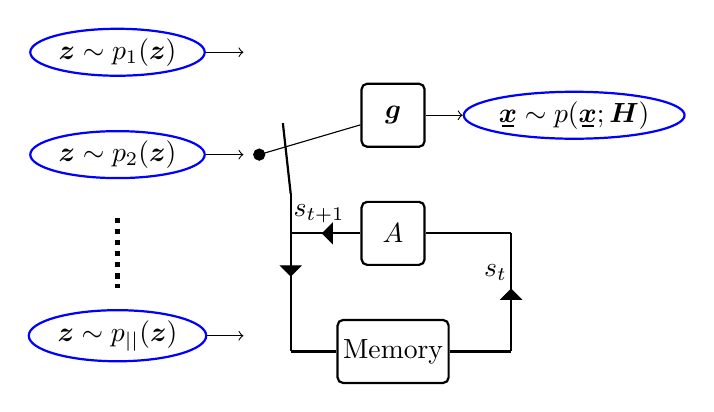
\begin{tikzpicture}
    \tikzstyle{enode} = [thick, draw=blue, ellipse, inner sep = 1pt,  align=center]
                                           %                                            \tikzstyle{nnode} = [thick, rectangle, rounded corners = 1pt,minimum size = 1.2cm,draw,inner sep = 2pt]
    \tikzstyle{nnode} = [thick, rectangle, rounded corners = 2pt,minimum size = 0.8cm,draw,inner sep = 2pt]
    \node[enode] (z1) at (0,1.8) {$\bm{z}\sim p_1(\bm{z})$};
    \node[enode] (z2) at (0,0.5){$\bm{z}\sim p_{2}(\bm{z})$};
    \node[enode] (zK) at (0,-1.8) {$\bm{z}\sim p_{|\Ss|}(\bm{z})$}; 
    \node[enode] (x) at (5.8,1){$\ubm{x}\sim p(\ubm{x};\bm{H})$};
                                           %                                            \node at (3,-1){$p(\bm{z}) = \sum_k\pi_kp_k(\bm{z})$};
    \node[nnode] (g) at (3.5,1) {$\bm{g}$};

    \node[nnode] (m) at (3.5,-2) {Memory};
    \node[nnode] (a) at (3.5,-0.5) {${A}$};


    \draw[dotted,line width=2pt] (0,-0.3) -- (0,-1.2);
    \filldraw[->] (1.8, 0.5)circle (2pt) --  (g) ;
    \draw[->] (z1) -- (1.6, 1.8);
    \draw[->] (z2) -- (1.6, 0.5);
                                           %                                            \draw[->] (1,-0.5) -- (1.8, -0.5);
    \draw[->] (zK) -- (1.6, -1.8);
                                           %                                            \draw[->] (z1) [in=180,out=0]  to node[right]{$\pi_1$} (g);
                                           %                                            \draw[->] (z2) [in=180,out=0]  to node[above]{$\pi_2$} (g);
                                           %                                            \draw[->,dashed] (zK) [in=180,out=0]  to node[right]{$\pi_K$} (g);
    \draw[->] (g) to (x);
    \begin{scope}[ thick, every node/.style={sloped,allow upside down}]
      \draw (2.1,0.9)-- (2.2, 0.);
      \draw (2.2,0.)-- node {\midarrow} (2.2,-2);
      \draw (2.2,-2)-- (m);
      \draw (m)-- (5, -2);
      \draw (5, -2)-- node {\midarrow} (5 ,-0.5);
      \draw (5, -0.5) -- (a);
      \draw (a)-- node {\midarrow} (2.2, -0.5);
    \end{scope}
    \node at (4.8, -1) {$s_{t}$};
    \node at (2.56, -0.25) {$s_{t+1}$};

  \end{tikzpicture}
  \caption{LatM-HMM Model defined by $\bm{H} = \{\Ss, \bm{q}, A, p({\bm{x}}|{\bm{s}}; \bm{\Phi}) \}$}
  \vspace{0.1cm}
\end{figure}

\textcolor{blue}{to be continued...}

Alternatively, we can use a latent-source mixed HMM (LatM-HMM) where different latent source share the same generator functioning as feature mapping. Then the generator of the LatM-HMM is defined as
\begin{equation}
  \left\{\bm{g}| \bm{g}: \bm{z}\rightarrow \bm{x}, s \in \Ss, \bm{z}\sim p_{s}(\bm{z})\right\}.
\end{equation}
We use $\bm{f} = \bm{g}^{-1}$ to denote inverse of $\bm{g}$ and use $\bm{\theta}$ to denote the parameter set of $\bm{g}$. Then the conditional probability for LatM-HMM is modeled as
\begin{align}
  p(\bm{x} | s; \bm{\Phi})
  &= p_s(\bm{z}) \bigg| \det \left( \pd{\bm{z}}{\bm{x}} \right) \bigg| \nonumber \\
  &= p_s(\bm{f}(\bm{x})) \bigg| \det \left( \pd{\bm{f}(\bm{x})}{\bm{x}} \right) \bigg|
\end{align}

The parameter set for this model to be decide is $\bm{\Phi} = \left\{ \bm{\theta},  \bm{\omega}_s, \forall s\in \Ss\right\}$.
Then the problem in \autoref{eq:sub-gm} can be reformulated as:
\begin{align}
  &\umax{\bm{\Phi}} \Qq(\bm{\Phi}; \bm{H}^{\mathrm{old}}) \nonumber \\
  =&\umax{ \bm{\theta}, \bm{\omega}_s, \forall s\in \Ss} \sum_{r=1}^{R} \sum_{t=1}^{{T}^{(r)}-1} \sum_{\smtr{s}{t}{r}=1}^{|\Ss|}  p(\smtr{s}{t}{r}| \ubmr{x}{r}; \bm{H}^{\mathrm{old}}) \left[\log\,p_{\smtr{s}{t}{r}}(\bm{f}(\bmtr{x}{t}{r})) + \log\,\bigg| \det\, \left( \pd{\bm{f}(\bmtr{x}{t}{r})}{\bmtr{x}{t}{r}} \right) \bigg| \right].
\end{align}


\subsubsection{Generator Shared HMM (GSHMM)}


\textbf{To be continued}...


\section{On Implementation of acoustic signal}
Found a HMM python lib that basics provide needed API for us, see \href{https://hmmlearn.readthedocs.io/en/stable/index.html}{hmmlearn}. Saikat also has suggestion.


For problem \autoref{eq:sub-gm} we are going to use our generative models to solve. I have the following consideration to revised our LatMM and GenMM for this application:
\begin{itemize}
\item Use factorized model instead of additive mixture model, to make likelihood computation logarithm domain compatible; 
\item Use full EM fashion instead of mini-batch fashion for training: store generative model as old for EM, there are always two neural networks working, one old for probability evaluation and one new for optimization.
\end{itemize}

\section{On Implementation of Planning}
Refer to \cite{kurutach2018learning_plan} and its \href{https://github.com/thanard/causal-infogan}{experiments}.

\bibliographystyle{plain}

     %      \bibliography{bibliography}
\bibliography{myref}

     %      \appendix

     %      \input{section/sec-appendixA}
\end{document}


%%% Local Variables:
%%% mode: latex
%%% TeX-master: t
%%% End:
